\subsection{Analysis: Symbolic Execution}

As we have discussed in the previous subsection, there are two types of approaches when we speak about verification:
\begin{itemize}
    \item \definition{Static Analysis}. It analyzes the source code, and each analyzer targets a fixed set of hard-coded (pre-defined, not custom) properties. It is entirely automatic, and the output reports two types of results: safe (no issues) and unsafe (potential problems). Also, the \textbf{analysis is made on generic (or symbolic) inputs}.
    
    The properties that we have mentioned are safety properties, such as:
    \begin{itemize}
        \item No \emph{overflow} for integer variables
        \item No \emph{type errors}
        \item No \emph{null-pointer} dereferencing
        \item No \emph{out-of-bound} array accesses
        \item No \emph{race conditions}
        \item No \emph{useless assignments}
        \item No \emph{usage of undefined variables}
        \item No \emph{execution of specific paths}
    \end{itemize}
    
    \item Testing (dynamic analysis) is made at runtime and is related to the software's behavior during execution. The analysis is also made on specific inputs.
\end{itemize}
Using the static analysis, we can use the symbolic execution.

\begin{definitionbox}
    \definition{Symbolic Execution} (also symbolic evaluation) \textbf{analyses a program to determine what inputs cause each part of a program to execute}.
\end{definitionbox}

\noindent
The \textbf{symbolic execution} analyzes actual source code and \textbf{reachability} and \textbf{path feasibility} properties. It is automatic and may fail to explore all possible paths. Sometimes, it is used to support testing.

The checked properties by the static analysis can be of different types:
\begin{itemize}
    \item \definition{Reachability}. Does some program execution reach location $L$ (generic line of code) in S (source code)? With the reachability property, the symbolic execution tries:
    \begin{itemize}
        \item To \textbf{verify} that $L$ \textbf{cannot be reached};
        \item Or \textbf{spots the condition under which} $L$ \textbf{can be reached}.
    \end{itemize}
    For example, in the following code:
    \begin{lstlisting}
...
k:      try {
k+1:        ...
L-1:    } catch (e) {
L:          /* error */
...     }\end{lstlisting}
    Static analysis checks the reachability properties and verifies that $L$ cannot be reached, or discovers the condition under which $L$ can be reached.
    
    \item \definition{Path Feasibility}. Is the given path $p$ feasible? With the path feasibility property, the symbolic execution tries:
    \begin{itemize}
        \item To \textbf{verify} that $p$ \textbf{cannot be executed};
        \item Or \textbf{spots the condition under which} $p$ \textbf{can be executed}.
    \end{itemize}
    Then $p$ will be:
    \begin{equation*}
        p = < 0, 1, \dots, k, \dots, n >
    \end{equation*}
\end{itemize}
Symbolic execution \textbf{executes programs on symbolic values}. Each symbolic value has its \textbf{symbolic states}, which keep track of the variables' (symbolic) values. The inputs are initialized with symbolic (generic) values.

\highspace
In the following example we can see a complete example of symbolic execution. But before we do, let us introduce some \underline{\textbf{limitations}} of this methodology.
\begin{itemize}
    \item The \textbf{path conditions may be too complex for constraint solvers}. Because solvers are very good at checking linear constraints, but it is harder for them to reason about non-linear arithmetic, bit-wise operations, string manipulation, etc.
    
    \item It is \textbf{impossible} or \textbf{difficult to use when the number of paths to be explored is infinite} or \textbf{huge}. For example, unbounded loops give rise to infinite sets of paths. Although the set of paths is finite, checking all loops is expensive and impractical.
    
    \item Finally, there may be \textbf{external code}. Then the sources are not available, such as a precompiled library, or the behavior is unknown to the solver.
\end{itemize}
\begin{examplebox}
    \begin{enumerate}
        \item First we introduce the annotation:
        \begin{lstlisting}
void foo(int x, int y) {
    ...\end{lstlisting}
        \begin{center}
            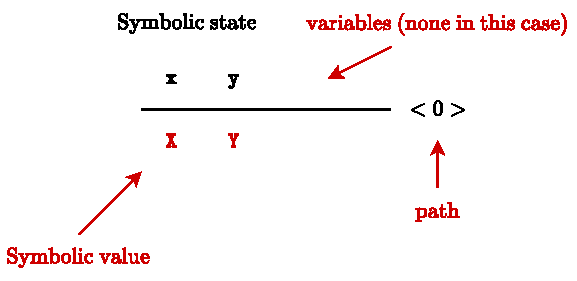
\includegraphics[width=.7\textwidth]{img/symbolic-state-1.pdf}
        \end{center}


        \item We introduce a local variable:
        \begin{lstlisting}
void foo(int x, int y) {
    int z := x\end{lstlisting}
        \begin{center}
            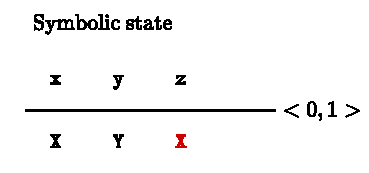
\includegraphics[width=.5\textwidth]{img/symbolic-state-2.pdf}
        \end{center}


        \item We introduce a condition. A \textbf{path condition} $\pi$ represents a constraint on a path:
        \begin{lstlisting}
void foo(int x, int y) {
    int z := x
    if (z < y)\end{lstlisting}
        \begin{itemize}
            \item if condition true
            \begin{center}
                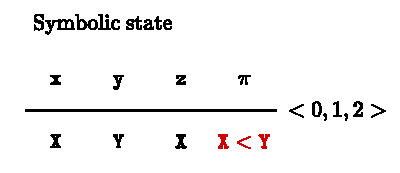
\includegraphics[width=.5\textwidth]{img/symbolic-state-3.pdf}
            \end{center}

            \item if condition false
            \begin{center}
                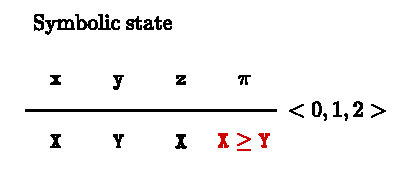
\includegraphics[width=.5\textwidth]{img/symbolic-state-4.pdf}
            \end{center}
        \end{itemize}


        \item \textbf{Execution continues along feasible paths}. In this case, the path condition $\pi$ is satisfiable:
        \begin{lstlisting}
void foo(int x, int y) {
    int z := x
    if (z < y)
        z := z*2\end{lstlisting}
        \begin{center}
            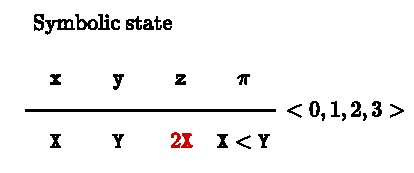
\includegraphics[width=.5\textwidth]{img/symbolic-state-5.pdf}
        \end{center}


        \item Another if condition:
        \begin{lstlisting}
void foo(int x, int y) {
    int z := x
    if (z < y)
        z := z*2
    if (x < y && z >= y)\end{lstlisting}
        \begin{itemize}
            \item if condition true
            \begin{center}
                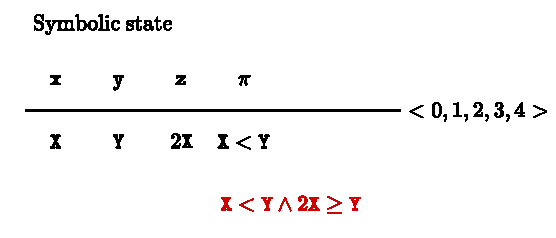
\includegraphics[width=.6\textwidth]{img/symbolic-state-6.pdf}
            \end{center}

            \item if condition false
            \begin{center}
                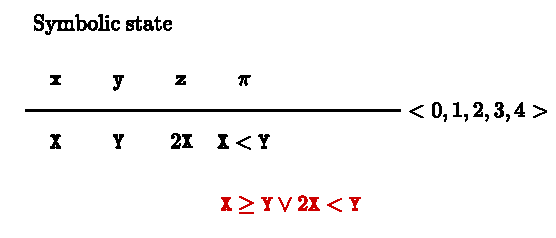
\includegraphics[width=.6\textwidth]{img/symbolic-state-7.pdf}
            \end{center}
        \end{itemize}


        \item Possible outcomes of symbolic execution:
        \begin{lstlisting}
void foo(int x, int y) {
    int z := x
    if (z < y)
        z := z*2
    if (x < y && z >= y)
        print(z)
}\end{lstlisting}
        \begin{enumerate}
            \item \textcolor{Green3}{\textbf{Satisfiable}} exit ($\pi$ is satisfiable): every satisfying assignment to variables in $\pi$ is an \textbf{input that satisfies the given property in a concrete execution}.
            \begin{center}
                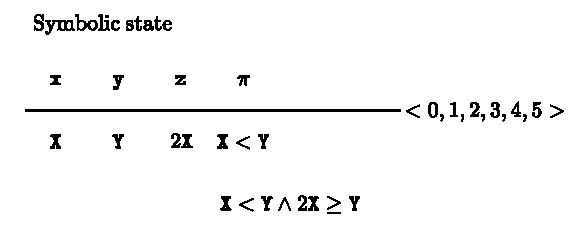
\includegraphics[width=.6\textwidth]{img/symbolic-state-8.pdf}
            \end{center}


            \item \textcolor{Red2}{\textbf{Unsatisfiable}} exit ($\pi$ is not satisfiable): the given \textbf{property cannot be satisfied by any concrete execution}.
            \begin{center}
                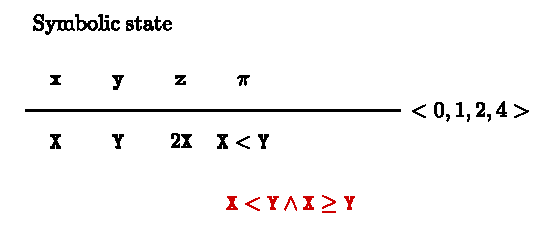
\includegraphics[width=.6\textwidth]{img/symbolic-state-9.pdf}
            \end{center}
        \end{enumerate}
    \end{enumerate}
    Finally, we can draw the \definition{Execution Tree}. The execution paths can be collected in an execution tree, where end states are marked as \texttt{SAT} or \texttt{UNSAT}.
    \begin{center}
        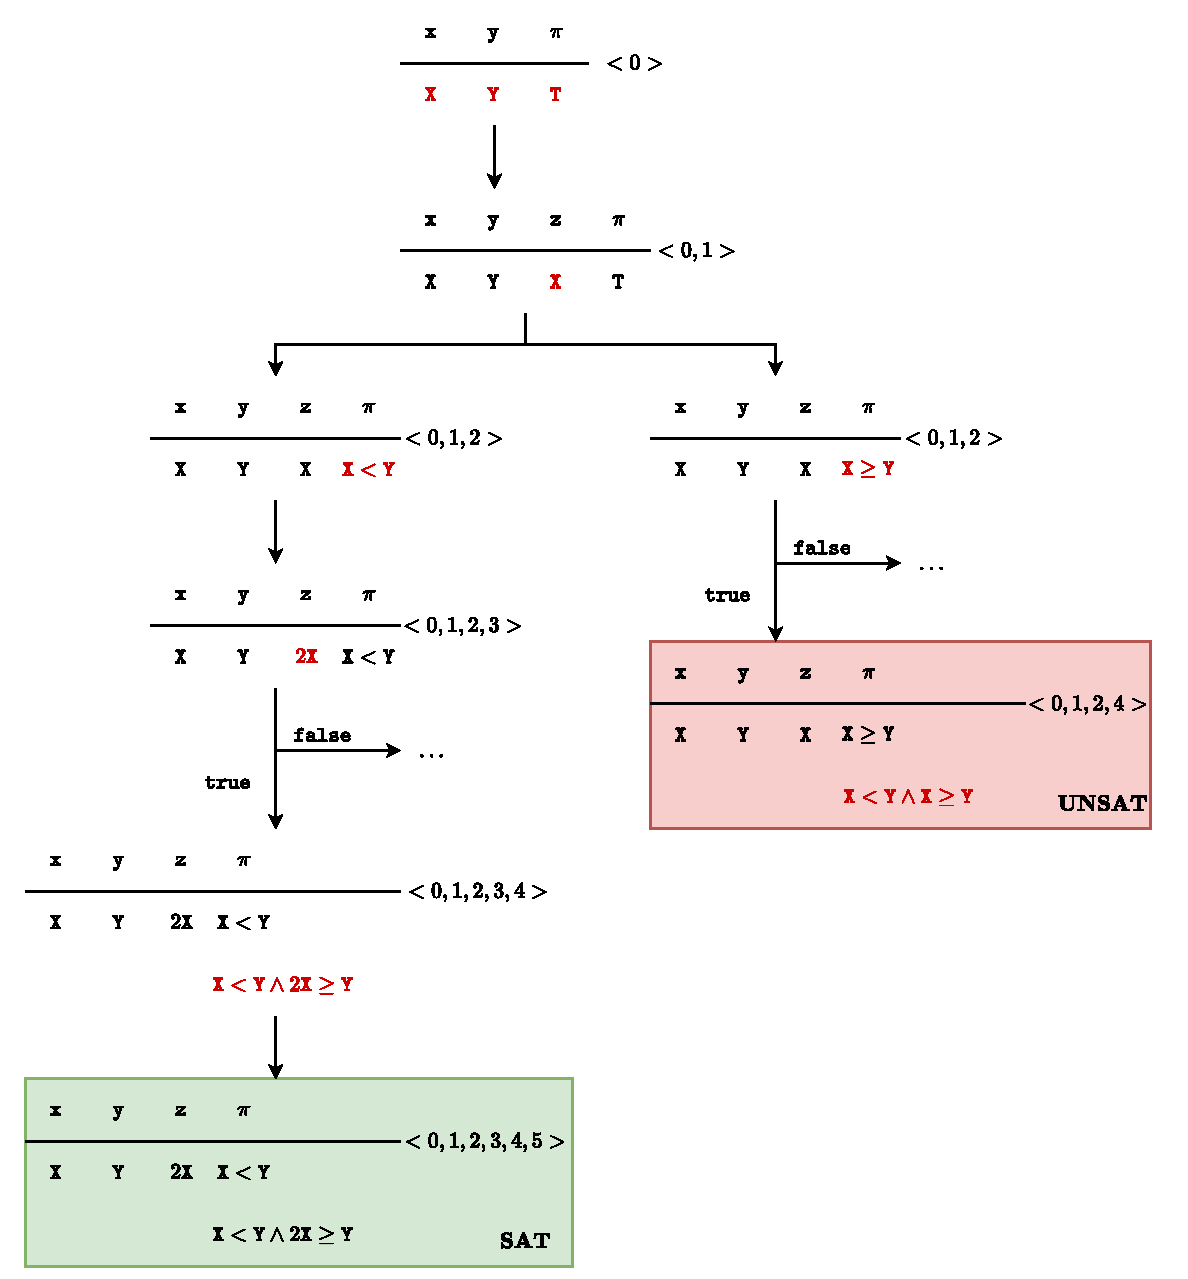
\includegraphics[width=\textwidth]{img/symbolic-state-10.pdf}
    \end{center}
    To view the tree in high resolution, scan (or click) the QR code below.
    \begin{center}
        \qrcode{https://github.com/PoliMI-HPC-E-notes-projects-AndreVale69/HPC-E-PoliMI-university-notes/tree/main/software-engineering-for-hpc/notes/img/symbolic-state-10.pdf}
    \end{center}
\end{examplebox}

\newpage

\subsection{Testing: terminology, types of testing activities}

\definition{Testing} (dynamic analysis) is an approach to verification. The \textbf{main goal of testing is to make programs fail}.

Other \emph{common goals} are:
\begin{itemize}
    \item Exercise different parts of a program to \textbf{increase coverage};
    
    \item Make sure the \textbf{interaction between components works} (\emph{integration testing});
    
    \item Support \textbf{fault localization} and \textbf{error removal} (\emph{debugging});
    
    \item Ensure that \textbf{bugs introduced in the past do not happen again} (\emph{regression testing}).
\end{itemize}
The dynamic analysis \textbf{analyzes program behavior}. The \textbf{properties} are \textbf{encoded as executable oracles representing expected outputs} and \textbf{desired conditions} (assertions).

It can \textbf{run only finite test cases}, so it's not exhaustive verification. The \textbf{failures have concrete inputs that trigger them}, and the \textbf{execution is automatic}.

\begin{flushleft}
    \textcolor{Green3}{\faIcon{question-circle} \textbf{We have often heard about \emph{debugging}, but what is it?}}
\end{flushleft}
\definition{Debugging} is a systematic approach to \textbf{fault localization and error removal}. The output is often used to support debugging.

\begin{figure}[!htp]
    \centering
    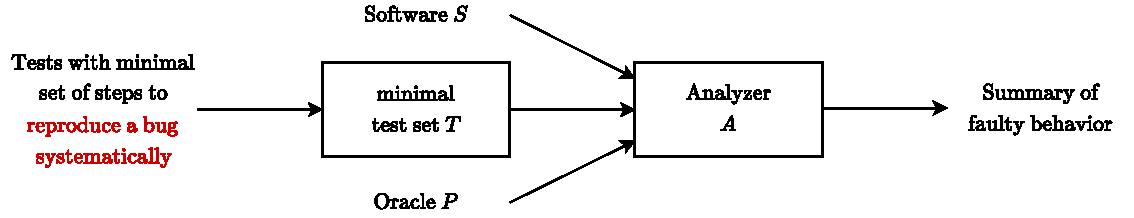
\includegraphics[width=\textwidth]{img/testing-1.pdf}
\end{figure}

\begin{flushleft}
    \textcolor{Green3}{\faIcon{question-circle} \textbf{... and \emph{test case}?}}
\end{flushleft}
\begin{definitionbox}
    A \definition{Test Case} is a set of \textbf{inputs}, \textbf{execution conditions}, and a \textbf{pass/fail criterion}.
\end{definitionbox}

\noindent
Running a test case typically involves setup, execution and teardown.
\begin{itemize}
    \item \textbf{Setup}. Bring the program to an \textbf{initial state} that fulfils the execution conditions.
    
    \item \textbf{Execution}. \textbf{Run} the program on the actual inputs.
    
    \item \textbf{Teardown}. \textbf{Record} the output, the final state, and any \textbf{failure} determined based on the pass/fail criterion.
\end{itemize}
A \textbf{test set}, or \textbf{test suite}, can include \textbf{multiple test cases}. Finally, a \definition{Test Case Specification} is a \textbf{requirement to be satisfied by one or more test cases}. An example of test case specification can be \emph{the input must be a sentence composed of at least two words}, and an example of test case input is \emph{this is a good test case input}.

\highspace
When discussing test cases, it's necessary to introduce \definition{Unit Testing}. This is \textbf{conducted by developers} and \textbf{aims to test small pieces} (units) \textbf{of code in isolation}. 

However, when we test in isolation, there should be a \textbf{problem}: the \textbf{units may depend on other units}. Then, we need to simulate missing units.

\highspace
The \definition{Integration Testing} (integration of the unit tests) \textbf{aims to exercise the interaction between interfaces and components}. The \textbf{faults} discovered by integration testing are multiple; some examples:
\begin{itemize}
    \item \textbf{Inconsistent interpretation of parameters} (e.g. mixed units meters or yards)

    \item \textbf{Violations of assumptions about domains} (e.g. buffer overflow)

    \item \textbf{Side effects on parameters or resources} (e.g. conflict on temporary file)

    \item \textbf{Nonfunctional properties} (e.g. unanticipated performance issues)

    \item \textbf{Concurrency-specific problems}
\end{itemize}
Typically, the integration test is defined by the Design Document. In the Design Document, we can find two types of plans:
\begin{itemize}
    \item \definition{Build Plan} that establishes the \textbf{order of the implementation};
    \item A \definition{Test Plan} that defines how to carry out integration testing is needed.
\end{itemize}
The strategies for the integration test are many:
\begin{itemize}
    \item \definition{Big Bang}: \textbf{test only after integrating all modules} (not even a real strategy). 
    
    \begin{flushleft}
        \textcolor{Green3}{\faIcon{check} \textbf{Pros}}
    \end{flushleft}
    It doesn't require stubs; it only \textbf{requires fewer drivers}/\textbf{oracles}.
    
    \begin{flushleft}
        \textcolor{Red2}{\faIcon{exclamation-triangle} \textbf{Cons}}
    \end{flushleft}
    \begin{enumerate}
        \item Minimum: observability, fault localization/diagnosability, efficacy, feedback;
        \item \textbf{High cost of repair} (cost of repairing a fault increases as a function of time between the introduction of an error in the code and repair).
    \end{enumerate}

    \newpage


    \item \definition{Iterative and incremental strategies}. The main action is \textbf{run after components are released (not just at the end)}. The strategy can be done in three different ways:
    \begin{itemize}
        \item \textbf{Hierarchical}. Based on the hierarchical structure of the system. It can be done top-down or bottom-up.
        \begin{itemize}
            \item \textbf{\emph{Top-down} strategy}. Work \textbf{from the top level} (in terms of \dquotes{use} or \dquotes{include} relationship) \textbf{down to the bottom level}. As modules are completed (according to the building plan), more functionality is testable. We also need to replace some stubs, and we need other stubs for lower levels. \textbf{When all modules are incorporated, the whole functionality can be tested}.
            
            \highspace
            \begin{flushleft}
                \textcolor{Green3}{\faIcon{check} \textbf{Pros}}
            \end{flushleft}
            The drivers use the top level interfaces (e.g. REST APIs).
            
            \highspace
            \begin{flushleft}
                \textcolor{Red2}{\faIcon{exclamation-triangle} \textbf{Cons}}
            \end{flushleft}
            This strategy requires stubs of used modules at each step of the process.

            \begin{figure}[!htp]
                \centering
                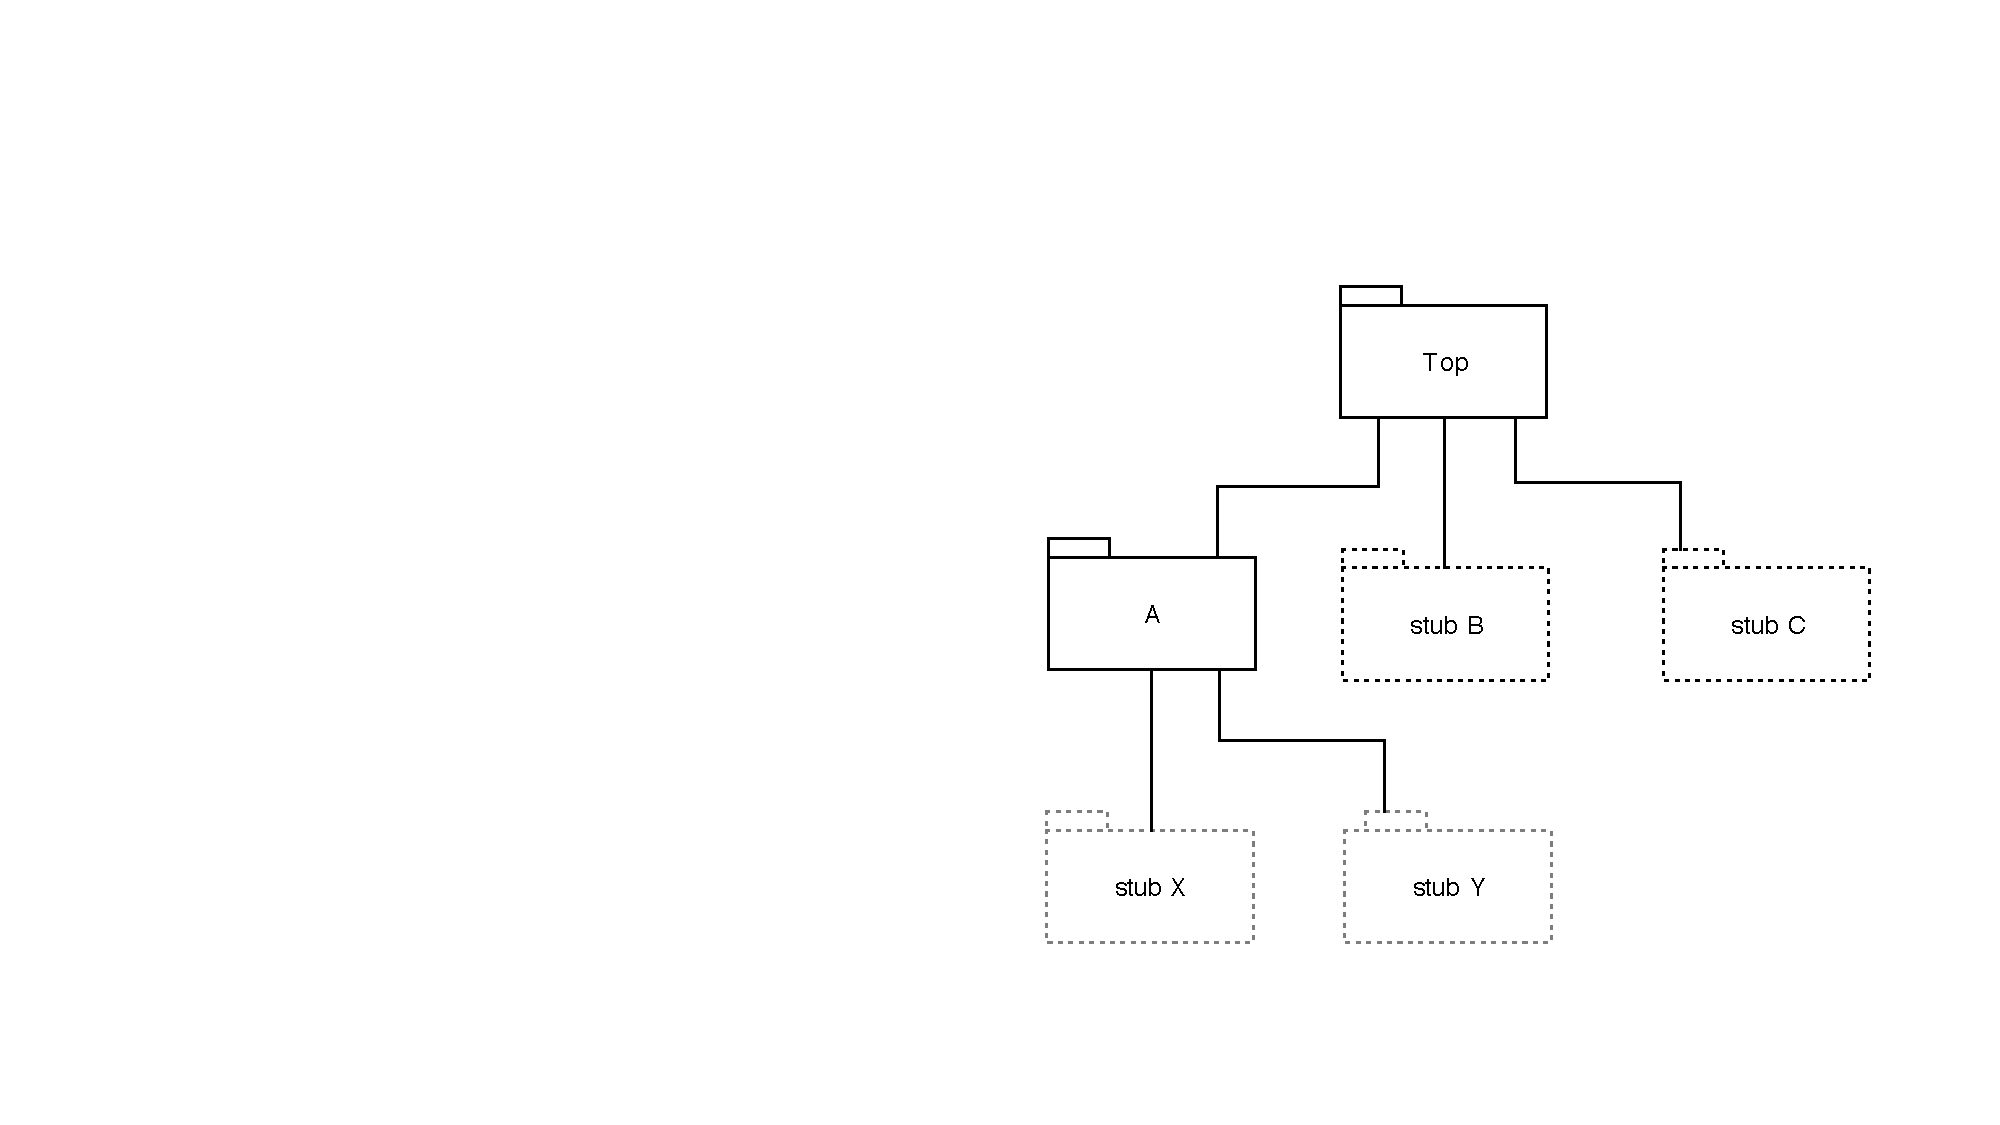
\includegraphics[width=.6\textwidth]{img/top-down-1.pdf}
                \caption{\example{Example} of top-down strategy.}
            \end{figure}
            
            \newpage

            \item \textbf{\emph{Bottom-up} strategy}. Starting from the leaves of the \dquotes{uses} hierarchy. 
            
            \highspace
            \begin{flushleft}
                \textcolor{Green3}{\faIcon{check} \textbf{Pros}}
            \end{flushleft}
            An advantage is that it \textbf{doesn't require stubs}.
            
            \highspace
            \begin{flushleft}
                \textcolor{Red2}{\faIcon{exclamation-triangle} \textbf{Cons}}
            \end{flushleft}
            \textbf{Typically requires more drivers} (one for each module, as in unit testing). Can this be a disadvantage? Maybe, because the newly developed module may replace an existing driver, and new modules require new drivers.

            Another thing to consider is that \textbf{it may create several working subsystems}, and each working subsystem will eventually be integrated into the final one.

            \begin{figure}[!htp]
                \centering
                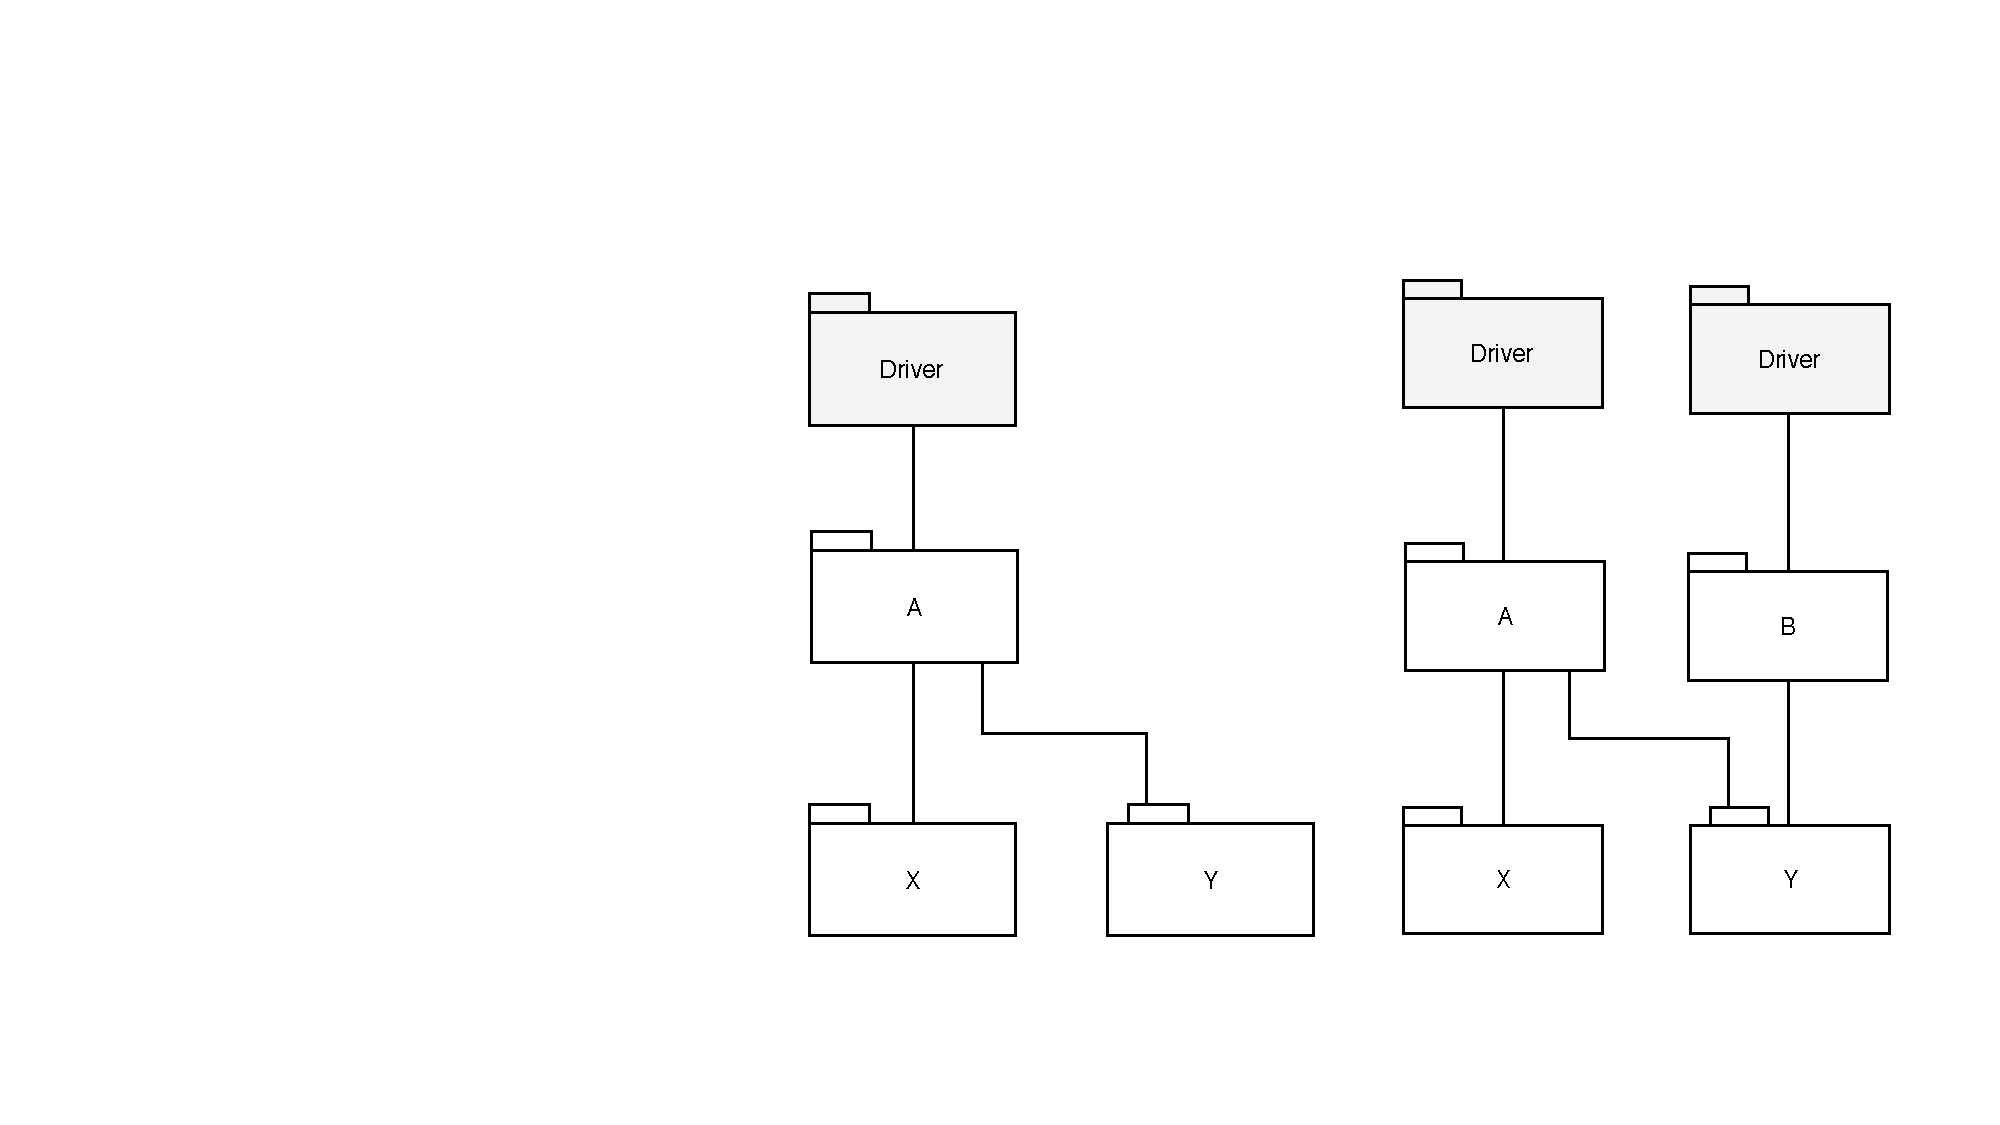
\includegraphics[width=.6\textwidth]{img/bottom-up-1.pdf}
                \caption{\example{Example} of bottom-up strategy.}
            \end{figure}
        \end{itemize}

        \newpage

        \item \textbf{Threads}. A \textbf{thread is a part of several modules that together provide a user-visible programme function}. By using the thread strategy we can have some \textbf{advantages}.
        \begin{flushleft}
            \textcolor{Green3}{\faIcon{check} \textbf{Pros}}
        \end{flushleft}
        \begin{itemize}
            \item We can \textbf{maximize the progress visible to the user} (or other stakeholders);
            \item \textbf{Reduce drivers and stubs};
            \item An integration plan is usually more complex.
        \end{itemize}
        \begin{figure}[!htp]
            \centering
            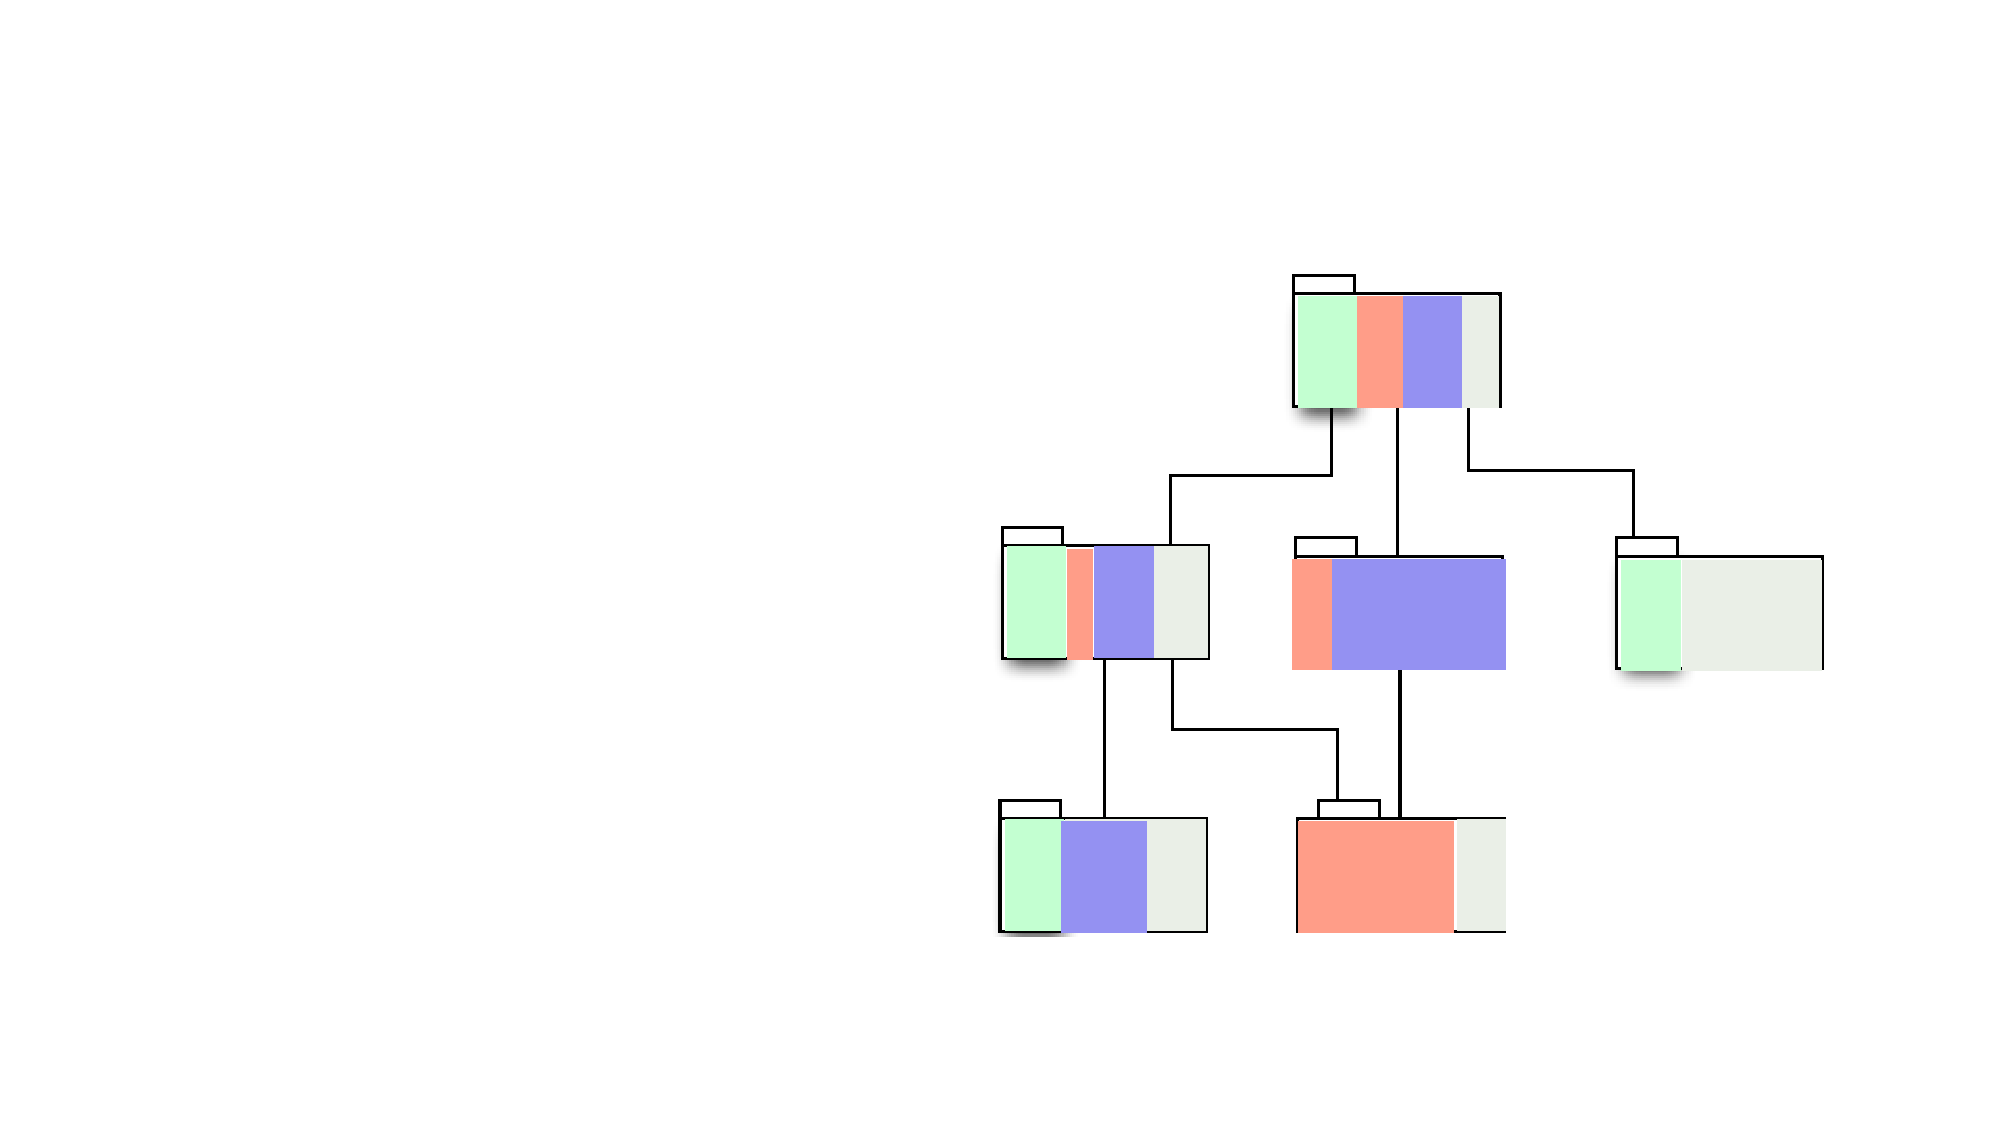
\includegraphics[width=.6\textwidth]{img/threads-1.pdf}
            \caption{\example{Example} of threads strategy.}
        \end{figure}
        
        \item \textbf{Critical}. The critical modules strategy \textbf{starts with the highest risk modules}. Risk assessment is a necessary first step. It can include technical risks (e.g. is X feasible?) and process risks (e.g. is the schedule for X realistic?). It may also be similar to a priority process.

        The \textbf{key point of this strategy is the risk-oriented process}. Integration and testing as a risk mitigation activity, designed to \emph{deliver any bad news as early as possible}.
    \end{itemize}
\end{itemize}

\begin{flushleft}
    \textcolor{Green3}{\faIcon{question-circle} \textbf{Which one should we choose?}}
\end{flushleft}
Given the three strategies above, \emph{which one should we choose}? Well, the structural strategies (bottom-up or top-down) are simpler, but thread and critical modules provide better external visibility of progress (especially in complex systems).

\highspace
So the \textbf{best choice} should be a \textbf{combination of different strategies}:
- Use \textbf{top-down/bottom-up} for relatively \textbf{small components} and \textbf{subsystems};
- Combinations of \textbf{thread} and \textbf{critical module integration testing} for \textbf{larger subsystems}.

\newpage

\subsubsection{E2E Testing}

\begin{definitionbox}
    \definition{End-to-end (E2E)} testing is a \textbf{software testing methodology to test a functional and data application flow consisting of several sub-systems working together from start to end}.\footnote{\href{https://microsoft.github.io/code-with-engineering-playbook/automated-testing/e2e-testing/}{Engineering Fundamentals Playbook}}
\end{definitionbox}

\noindent
At times, these systems are developed in different technologies by different teams or organizations. Finally, they come together to form a functional business application. Hence, testing a single system would not suffice. Therefore, end-to-end testing verifies the application from start to end putting all its components together.

\highspace
The following is a list of \textbf{common types of tests} that use the E2E system:
\begin{itemize}
    \item \definition{Functional Testing}
    \begin{flushleft}
        \textcolor{Red2}{\faIcon{book} \textbf{Purpose}}
    \end{flushleft}
    Check whether the \textbf{software meets the functional requirements}.

    \begin{flushleft}
        \textcolor{Green3}{\faIcon{question-circle} \textbf{How?}}
    \end{flushleft}
    Use the software as described by use cases in the RASD (pag. \pageref{RASD}), check whether requirements are fulfilled.


    \item \definition{Performance Testing}
    \begin{flushleft}
        \textcolor{Red2}{\faIcon{book} \textbf{Purpose}}
    \end{flushleft}
    \begin{enumerate}
        \item Detect \textbf{bottlenecks} affecting response time, utilization, throughput
        \item Detect \textbf{inefficient algorithms}
        \item Detect \textbf{hardware/network issues}
        \item Identify \textbf{optimization possibilities}
    \end{enumerate}

    \begin{flushleft}
        \textcolor{Green3}{\faIcon{question-circle} \textbf{How?}}
    \end{flushleft}
    Load the system with the expected workload and measure and compare acceptable performance.
    
    \newpage

    \item \definition{Load Testing}
    \begin{flushleft}
        \textcolor{Red2}{\faIcon{book} \textbf{Purpose}}
    \end{flushleft}
    \begin{enumerate}
        \item \textbf{Expose bugs} such as memory leaks, mismanagement of memory, buffer overflows
        \item Identify \textbf{upper limits of components}
        \item \textbf{Compare alternative architectural options}
    \end{enumerate}

    \begin{flushleft}
        \textcolor{Green3}{\faIcon{question-circle} \textbf{How?}}
    \end{flushleft}
    Test the system at increasing workload until it can support it, and load the system for a long period.


    \item \definition{Stress Testing}
    \begin{flushleft}
        \textcolor{Red2}{\faIcon{book} \textbf{Purpose}}
    \end{flushleft}
    Make sure that the \textbf{system recovers gracefully after failure}.

    \begin{flushleft}
        \textcolor{Green3}{\faIcon{question-circle} \textbf{How?}}
    \end{flushleft}
    Trying to break the system under the test by overwhelming its resources or by reducing resources.

    For \example{example} double the baseline number for concurrent users/HTTP connections, or randomly shut down and restart ports on the network switches/routers that connect servers.
\end{itemize}